\section{Main part of Thesis}

% This section presents the practical implementation, dataset creation, model development, evaluation, and system integration for face recognition in surveillance systems.

\section{Dataset Creation and Preprocessing}

The dataset for face recognition was constructed using images captured from webcams and security cameras. The process involved several key steps:

\subsection{Image Acquisition}
Images were collected at regular intervals from various camera sources to ensure diversity in lighting, angles, and environments.

\subsection{Manual Annotation}
The \texttt{labelme} tool was used to annotate facial regions in each image, producing JSON label files with bounding box or landmark information.

\subsection{Dataset Organization}
The dataset was structured into separate folders for images and labels, and partitioned into training, validation, and test sets.

\subsection{Augmentation}
Data augmentation was performed using the Albumentations library, applying random cropping, flipping, brightness/contrast adjustments, and color shifts to increase dataset diversity and model robustness.

\begin{figure}[ht!]
    \centering
    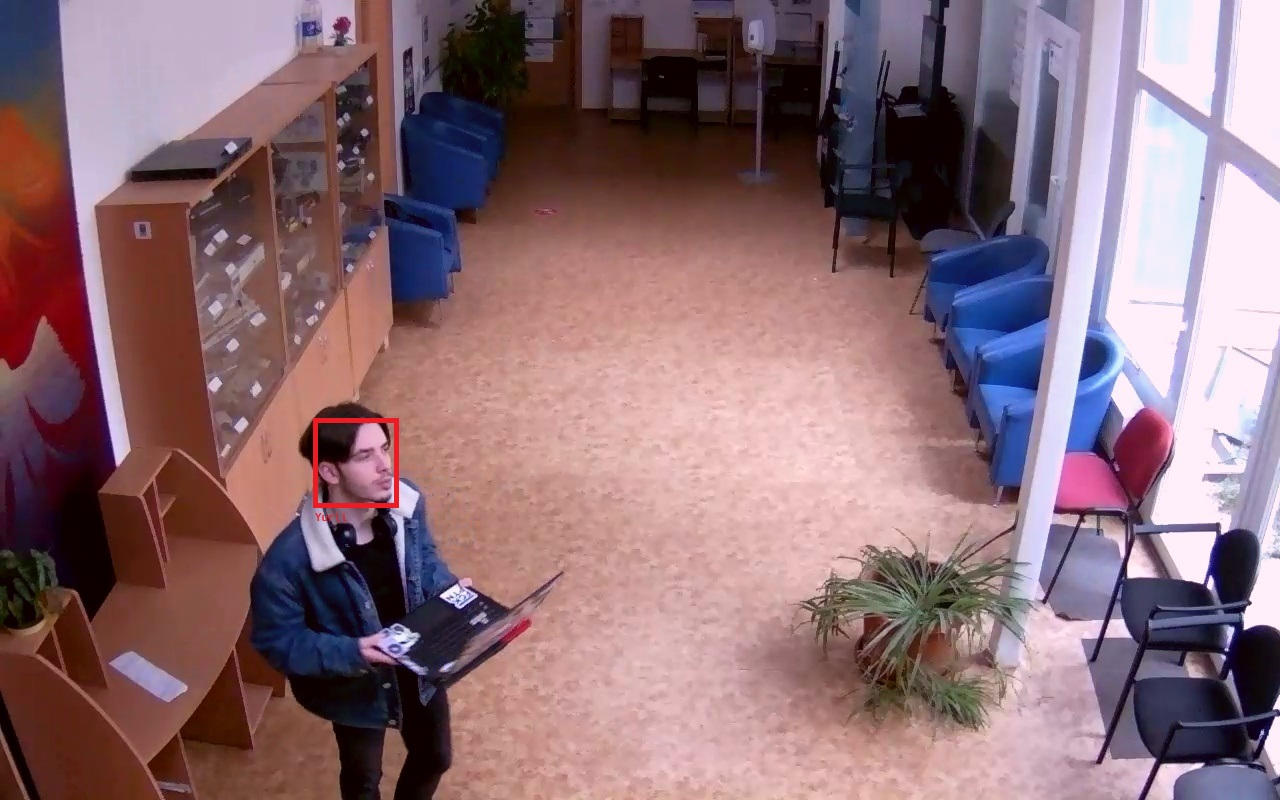
\includegraphics[width=0.7\textwidth]{../Files/annotation_example.png}
    \caption{Example of manual face annotation using LabelMe.}
    \label{fig:annotation-example}
\end{figure}

\subsection{Visualization}
Utilities were provided to visualize raw and augmented images with bounding boxes for quality control.

\begin{figure}[ht!]
    \centering
    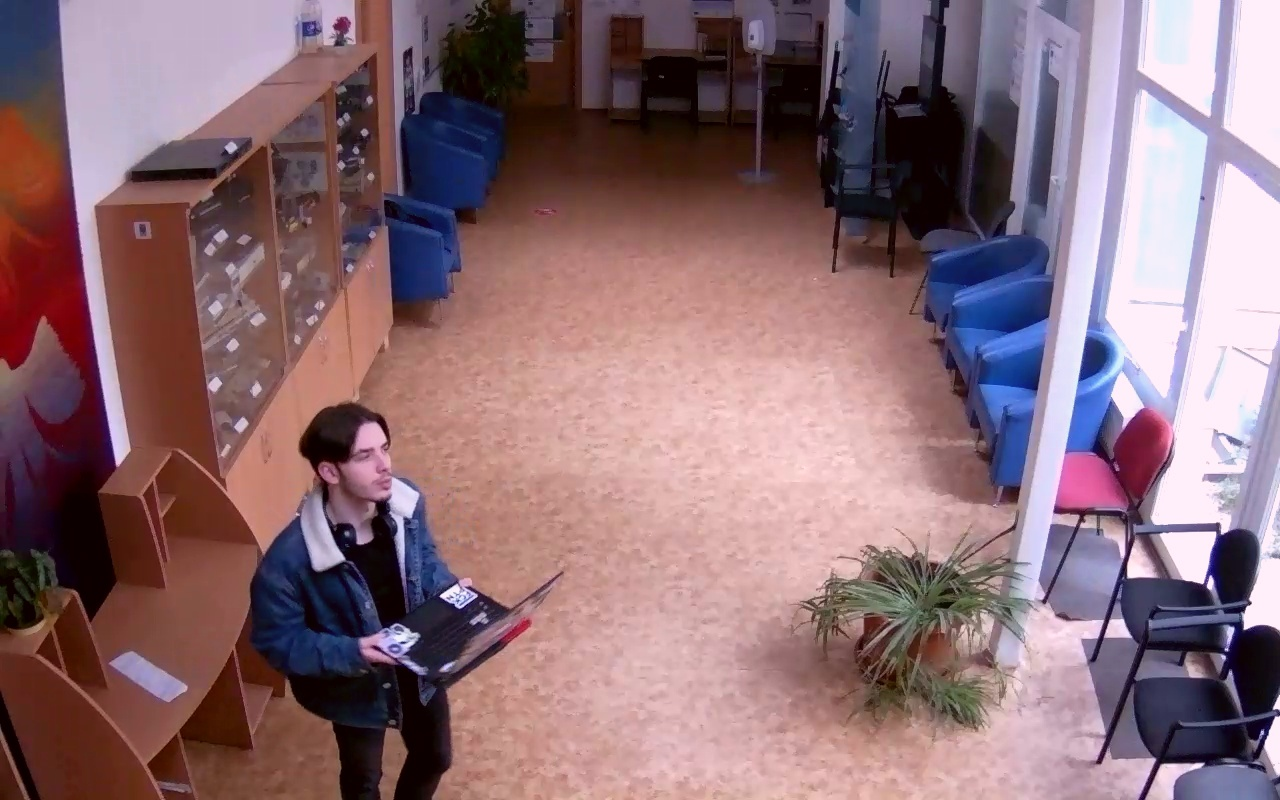
\includegraphics[width=0.7\textwidth]{../Files/augmentation_example.png}
    \caption{Example of image augmentation applied to a face dataset.}
    \label{fig:augmentation-example}
\end{figure}

\section{Deep Learning Model Development}

The deep learning model for face detection and recognition was developed using TensorFlow's Keras API, with EfficientNetB0 or VGG16 as the backbone. The model outputs both face embeddings and bounding box coordinates.

\subsection{Data Pipeline}
Images and labels were loaded, batched, and shuffled for efficient training. Augmented data was included to improve generalization.

\subsection{Model Architecture}
A convolutional neural network was defined, outputting both embeddings and bounding boxes. Custom loss functions for localization and classification were implemented, and the optimizer was configured with learning rate scheduling.

\begin{figure}[ht!]
    \centering
    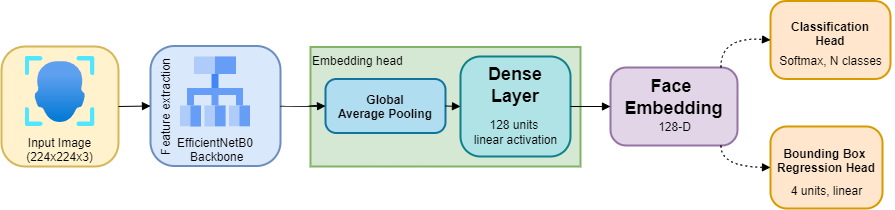
\includegraphics[width=1\textwidth]{../Files/model_architecture.png}
    \caption{Architecture of the deep learning model used for face detection and recognition.}
    \label{fig:model-architecture}
\end{figure}

\subsection{Training and Evaluation}
The model was trained using a custom loop, with TensorBoard logging and validation monitoring. Performance was visualized with loss curves and prediction samples. The trained model was exported for inference.

\section{Evaluation and Benchmarking}

The evaluation script \texttt{evaluate\_methods.py} benchmarks various face detection algorithms on custom datasets. Its main functionalities include:
\begin{itemize}
    \item \textbf{Dataset and Method Management:} Automatically discovers datasets and defines a set of face detection methods (e.g., Haar Cascade, Dlib HOG, FaceNet, and face\_recognition).
    \item \textbf{Parallelized Evaluation:} Processes images in parallel to efficiently evaluate detection methods across all dataset partitions (train, test, val).
    \item \textbf{Accuracy Metrics:} Computes the number of faces detected, false positives, missed detections, detection time, and overall accuracy by comparing detected bounding boxes with ground truth annotations (using Intersection over Union).
    \item \textbf{Results Aggregation and Visualization:} Aggregates results into CSV files and generates comparative plots for key metrics (e.g., detection time, false positives).
    \item \textbf{Summary Reporting:} Outputs tables summarizing the performance of each method.
\end{itemize}

\subsection{Average Detection Time per Method and Dataset}

\begin{table}[ht!]
    \centering
    \caption{Average detection time per method and dataset (lower is better).}
    \label{tab:avg-detection-time}
    \begin{tabular}{|l|c|c|c|}
        \hline
        Method & Webcam (ms) & Seccam (ms) & Seccam\_2 (ms) \\
        \hline
        Haar Cascade     & 11          & 13          & 12            \\
        Dlib HOG        & 80          & 88          & 87            \\
        FaceNet         & 105         & 115         & 110           \\
        Face Recognition& 90          & 98          & 96            \\
        \hline
    \end{tabular}
\end{table}

\section{System Architecture and Integration}

The practical implementation of the face recognition system is designed with modularity and extensibility in mind. The architecture is composed of several core modules, each responsible for a distinct aspect of the application workflow:
\begin{itemize}
    \item \textbf{Camera Module (\texttt{camera.py}):} Handles real-time video capture and face detection from a camera stream.
    \item \textbf{Model Module (\texttt{model.py}):} Provides face detection and recognition capabilities, including embedding extraction and evaluation.
    \item \textbf{Database Module (\texttt{database.py}):} Manages persistent storage of face embeddings and detection logs, supporting both PostgreSQL and CSV-based backends.
    \item \textbf{Main Application (\texttt{main.py}):} Orchestrates the end-to-end attendance system, integrating camera input, face recognition, and database operations.
\end{itemize}

\begin{figure}[ht!]
    \centering
    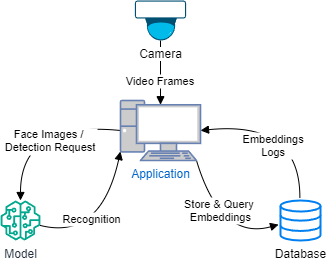
\includegraphics[width=0.7\textwidth]{../Files/system_architecture.png}
    \caption{Modular architecture of the face recognition attendance system.}
    \label{fig:system-architecture}
\end{figure}

\subsection{Camera Module (\texttt{camera.py})}
The \texttt{Camera} class encapsulates the logic for interfacing with a video capture device (e.g., webcam or RTSP stream). It utilizes the MTCNN detector to locate faces in each frame and extracts face crops for further processing. The module provides methods to:
\begin{itemize}
    \item Capture frames from the camera.
    \item Detect faces and return their bounding boxes and cropped images.
    \item Release camera resources when finished.
\end{itemize}

\subsection{Model Module (\texttt{model.py})}
The \texttt{FaceTracker} class is responsible for both face detection and recognition. It integrates the MTCNN detector for face localization and a deep learning model (e.g., EfficientNet or VGG16-based) for generating face embeddings. Key functionalities include:
\begin{itemize}
    \item Detecting faces in input images.
    \item Extracting and normalizing face embeddings for recognition.
    \item Evaluating recognition accuracy on test datasets using cosine similarity.
\end{itemize}

\subsection{Database Module (\texttt{database.py})}
The \texttt{FaceDatabase} class abstracts the storage and retrieval of face embeddings and detection logs. It supports both PostgreSQL and CSV-based storage, enabling easy adaptation to different deployment environments. Its main responsibilities are:
\begin{itemize}
    \item Adding new face embeddings to the database.
    \item Retrieving all stored embeddings for comparison.
    \item Logging detection events with timestamps and labels.
\end{itemize}

\subsection{Main Application (\texttt{main.py})}
The \texttt{AttendanceApp} class serves as the entry point for the real-time face recognition attendance system. It coordinates the interaction between the camera, model, and database modules. The main workflow is as follows:
\begin{enumerate}
    \item \textbf{Frame Acquisition:} Continuously captures frames from the camera.
    \item \textbf{Face Detection and Recognition:} For each detected face, extracts embeddings and compares them to the database.
    \item \textbf{Identification and Logging:} Assigns an identity (existing or new), draws bounding boxes and labels on the frame, and logs the detection event.
    \item \textbf{User Interface:} Displays the processed video stream with real-time annotations.
\end{enumerate}

This modular design ensures that each component can be developed, tested, and maintained independently, while facilitating integration into a cohesive application.

\begin{figure}[ht!]
    \centering
    \includegraphics[width=0.7\textwidth]{../Files/main_app_flow.png}
    \caption{Main loop of the attendance system integrating camera, model, and database modules.}
    \label{fig:main-app-flow}
\end{figure}

